\section{Introduction}

This chapter presents experimental results and an evaluation of the
performance of OmniTune when tasked with selecting workgroup size of
SkelCL stencil codes. The effectiveness of each of the autotuning
techniques described in the previous chapters are evaluated using
multiple different machine learning algorithms, and the prediction
quality is scrutinised for portability across programs, devices, and
datasets.


% \subsubsection{Questions to ask of each approach to autotuning}
%
% \item What is the performance when testing on an unseen:
%   architecture, kernel, dataset? (leave one out evaluation)
% \item How well does it perform as a function of the number of
%   training points?
% \end{enumerate}


\section{Statistical Soundness}


\begin{figure}
  \centering
\begin{subfigure}[h]{.45\textwidth}
  \centering
  \includegraphics{gen/img/num_samples}
  \caption{}
\end{subfigure}
\hfill
\begin{subfigure}[h]{.45\textwidth}
  \centering
  \includegraphics{gen/img/num_params}
  \caption{}
\end{subfigure}

  \caption{%
    Coverage reports for the first 100: (\subref{fig:sample-counts})
    samples per test case; (\subref{fig:param-counts}) workgroup sizes
    per scenario.%
  }
\label{fig:num-samples}
\end{figure}

A total of \input{gen/num_runtime_stats} \emph{test cases} were
evaluated, where a test case $t_i$ is a scenario, workgroup size pair
$t_i = (s_i,w_i)$. This represents an exhaustive enumeration of the
legal workgroup sizes for \input{gen/num_scenarios} scenarios, with an
average of \input{gen/avg_num_params} (max \input{gen/max_num_params})
unique workgroup sizes each. Figures~\ref{fig:sample-counts}
and~\ref{fig:param-counts} show the number of samples per test case
and unique workgroup sizes per scenario respectively.


\begin{figure}
\begin{subfigure}[h]{.32\textwidth}
\centering
\includegraphics{gen/img/runtimes_histogram_1}
\vspace{-1.5em} % Shrink vertical padding
\caption{}
\label{fig:runtimes-histogram-1}
\end{subfigure}
~%
\begin{subfigure}[h]{.32\textwidth}
\centering
\includegraphics{gen/img/runtimes_histogram_2}
\vspace{-1.5em} % Shrink vertical padding
\caption{}
\label{fig:runtimes-histogram-2}
\end{subfigure}
~%
\begin{subfigure}[h]{.32\textwidth}
\centering
\includegraphics{gen/img/runtimes_histogram_3}
\vspace{-1.5em} % Shrink vertical padding
\caption{}
\label{fig:runtimes-histogram-3}
\end{subfigure}
\\
\begin{subfigure}[h]{.32\textwidth}
\centering
\includegraphics{gen/img/runtimes_histogram_4}
\vspace{-1.5em} % Shrink vertical padding
\caption{}
\label{fig:runtimes-histogram-4}
\end{subfigure}
~%
\begin{subfigure}[h]{.32\textwidth}
\centering
\includegraphics{gen/img/runtimes_histogram_5}
\vspace{-1.5em} % Shrink vertical padding
\caption{}
\label{fig:runtimes-histogram-5}
\end{subfigure}
~%
\begin{subfigure}[h]{.32\textwidth}
\centering
\includegraphics{gen/img/runtimes_histogram_6}
\vspace{-1.5em} % Shrink vertical padding
\caption{}
\label{fig:runtimes-histogram-6}
\end{subfigure}
\\
\begin{subfigure}[h]{.32\textwidth}
\centering
\includegraphics{gen/img/runtimes_histogram_7}
\vspace{-1.5em} % Shrink vertical padding
\caption{}
\label{fig:runtimes-histogram-7}
\end{subfigure}
~%
\begin{subfigure}[h]{.32\textwidth}
\centering
\includegraphics{gen/img/runtimes_histogram_8}
\vspace{-1.5em} % Shrink vertical padding
\caption{}
\label{fig:runtimes-histogram-8}
\end{subfigure}
~%
\begin{subfigure}[h]{.32\textwidth}
\centering
\includegraphics{gen/img/runtimes_histogram_9}
\vspace{-1.5em} % Shrink vertical padding
\caption{}
\label{fig:runtimes-histogram-9}
\end{subfigure}

\caption{%
  Distribution of runtime samples for 9 test cases with average
  runtimes between 2-200ms. Each plot contains a 35-bin histogram of
  1000 samples, and a fitted kernel density estimate with bandwidth
  0.3. The sample mean is shown as a vertical dashed line.%
}
\label{fig:runtime-histograms}
\end{figure}


\begin{figure}
\centering
\includegraphics{gen/img/ci_trend}
\caption{%
  % FIXME: Check against \input{gen/max_ci} and \input{gen/mean_ci}
  Ratio of confidence interval to mean as a function of sample
  count. The two dashed lines indicate the confidence interval at the
  minimum sample count (\fixme{4.5}\%), and mean sample count
  (\fixme{2.6}\%).%
}
\label{fig:ci-trends}
\end{figure}


For each test case, an average of \input{gen/avg_sample_count} samples
were recorded (min \input{gen/min_sample_count}, total
\input{gen/num_samples}). Applying the central limit theorem allows us
to assume an underlying Gaussian distribution of
samples~\cite{Georges2007}. To test this, a random subset of 1000 test
cases were chosen and 1000 samples recorded for
each. Figure~\ref{fig:runtime-histograms} shows fine-grained
histograms of all sampled runtimes for 9 of those test cases, with
mean runtimes between 2-200ms. Assuming a normal distribution, 95\%
confidence intervals can be used to provide statistical confidence of
a sample mean with respect to the true
mean. Figure~\ref{fig:ci-trends} plots 95\% confidence intervals
(normalised to their respective means) as a function of the number of
samples for these 1000 test cases, showing diminishing returns as the
number of samples increase. By comparing the average confidence
interval at different sample counts against the complete dataset of
\input{gen/num_runtime_stats} test cases, we can assert with 95\%
confidence that the true mean for each test case is within
\input{gen/mean_ci}\% of our sample mean (given the average number of
samples per test case), or \input{gen/max_ci}\% in the worst case (at
the minimum number of samples). \FIXME{It seems like it'd be a good
  idea to add a normality test.}


\section{Optimising Workgroup Sizes}



\cleardoublepage
\begin{figure}
\begin{subfigure}[h]{\textwidth}
\centering
\includegraphics{gen/img/performance_max_wgsize}
\vspace{-1.5em} % Shrink vertical padding
\caption{}
\label{fig:performance-max-wgsize}
\end{subfigure}
\\
\begin{subfigure}[h]{.48\textwidth}
\centering
\includegraphics{gen/img/performance_max_c}
\vspace{-1.5em} % Shrink vertical padding
\caption{}
\label{fig:performance-wg-c}
\end{subfigure}
~%
\begin{subfigure}[h]{.48\textwidth}
\centering
\includegraphics{gen/img/performance_max_r}
\vspace{-1.5em} % Shrink vertical padding
\caption{}
\label{fig:performance-wg-r}
\end{subfigure}

\caption{%
  Comparing workgroup performance relative to the oracle as function
  of: (\subref{fig:performance-max-wgsize})~maximum legal size,
  (\subref{fig:performance-wg-c})~number of columns, and
  (\subref{fig:performance-wg-r})~ number of rows.%
}
\label{fig:performance-wgsizes}
\end{figure}
\newpage
\begin{figure}
\begin{subfigure}[h]{\textwidth}
\centering
\includegraphics{gen/img/performance_kernels.pdf}
\vspace{-1.5em} % Shrink vertical padding
\caption{Kernels}
\label{fig:performance-kernels}
\end{subfigure}
\\
\begin{subfigure}[h]{.48\textwidth}
\centering
\includegraphics{gen/img/performance_devices.pdf}
\vspace{-1.5em} % Shrink vertical padding
\caption{Devices}
\label{fig:performance-devices}
\end{subfigure}
~%
\begin{subfigure}[h]{.48\textwidth}
\centering
\includegraphics{gen/img/performance_datasets.pdf}
\vspace{-1.5em} % Shrink vertical padding
\caption{Datasets}
\label{fig:performance-datasets}
\end{subfigure}

\caption{%
  Performance relative to the oracle of workgroup sizes across all
  test cases, grouped by: (\subref{fig:performance-kernels})~kernels,
  (\subref{fig:performance-devices})~devices, and
  (\subref{fig:performance-datasets})~datasets.%
}
\label{fig:performances}
\end{figure}

% To begin to get a feel for the
%
% Figure~\ref{fig:performance-wgsizes}. Furthermore, the performance of
% workgroup sizes is shown in Figure~\ref{fig:performances} to be vary
% greatly across architectures, kernels, and datasets.

\TODO{What is the distribution of relative performance across
  architectures, programs, and datasets?}

\begin{table}
  \parbox{.45\linewidth}{
    \centering
    \scriptsize
    \rowcolors{2}{white}{gray!25}
    \input{gen/tab/top_params_coverage}
    \caption{The 25 workgroup sizes with the greatest legality.}
  }
  \hfill
  \parbox{.45\linewidth}{
    \centering
    \scriptsize
    \rowcolors{2}{white}{gray!25}
    \input{gen/tab/top_params_perf}
    \caption{The 25 workgroup sizes with the greatest performance.}
  }
\end{table}


\begin{figure}
\centering
\includegraphics{gen/img/params_summary.pdf}
\caption{%
  The red line shows the ``legality'' of workgroup sizes, i.e.\ the
  ratio of scenarios for which that workgroup size is legal.  The
  green lines show the geometric mean of the performance relative to
  the oracle for all scenarios for which the workgroup size is legal.%
}
\label{fig:performance-legality}
\end{figure}


\subsection{Performance Upper Bounds}

\begin{figure}
\includegraphics{gen/img/max_speedups}
\caption{%
  Speedup of oracle workgroup size over the worst workgroup size for
  each scenario, and the statically chosen workgroup size that
  provides the best overall performance.%
}
\label{fig:speedups}
\end{figure}

For a given scenario $s$, the ratio of the workgroups sizes from
$W_{legal}(s)$ which provide the longest and shortest mean runtimes is
used to calculate an upper bound for the possible performance
influence of workgroup size:

\begin{equation}
r_{max}(s) = r(s, \argmax_{w \in W_{legal}(s)} t(s,w), \Omega(s))
\end{equation}

When applied to each scenario $s \in S$ from the experimental results,
the average performance upper bound is found to be
$\input{gen/avg_possible_speedup}\times$ (range:
$\input{gen/min_possible_speedup}\times$ -
$\input{gen/max_possible_speedup}\times$).

\TODO{T-test to demonstrate confidence in differences between best and
  worst params.}


\subsection{Refused Parameters}

Of the \input{gen/num_params} workgroup sizes tested,
\input{gen/ratio_refused_params}\% were refused in one or more test
cases, with an average \input{gen/ratio_refused_test_cases}\% of test
cases leading to refused parameters. For a workgroup size to be
refused, it must satisfy the architectural and program-specific
constraints which are exposed by OpenCL, but still lead to a
\texttt{CL\_OUT\_OF\_RESOURCES} error when the kernel is
enqueued. Table~\ref{tab:top-refused-params} lists the most frequently
refused parameters, and the percentage of test cases for which they
were refused. While uncommon, a refused parameters is an obvious
inconvenience to the user, as one would expect that any workgroup size
within the specified maximum should behave \emph{correctly} if not
performantly.

Figure~\ref{fig:refused-params-by-dev-vendor} suggests that the
problem is vendor --- or at least device --- specific. The
distribution of refused parameters is skewed towards the Intel CPU
devices, while no workgroup sizes were refused by the AMD
GPU. \TODO{Bug reports\ldots} For now, it is imperative that the
autotuning system be capable of adapting to these refused parameters
by suggesting alternatives when they occur.

\begin{table}
\parbox{.32\linewidth}{
    \centering
    \scriptsize
    \rowcolors{2}{white}{gray!25}
    \input{gen/tab/top_refused_params_1}
  }
  \hfill
  \parbox{.32\linewidth}{
    \centering
    \scriptsize
    \rowcolors{2}{white}{gray!25}
    \input{gen/tab/top_refused_params_2}
  }
  \hfill
  \parbox{.32\linewidth}{
    \centering
    \scriptsize
    \rowcolors{2}{white}{gray!25}
    \input{gen/tab/top_refused_params_3}
  }
  \caption{The thirty most refused parameters, ranked in descending
    order.}
  \label{tab:top-refused-params}
\end{table}

\begin{figure}
\centering
\begin{subfigure}[h]{.45\textwidth}
  \centering
  \includegraphics{gen/img/refused_params_by_device}
  \caption{}
  \label{fig:refused-params-by-device}
\end{subfigure}
\hfill
\begin{subfigure}[h]{.45\textwidth}
  \centering
  \includegraphics{gen/img/refused_params_by_vendor}
  \caption{}
  \label{fig:refused-params-by-vendor}
\end{subfigure}
\caption{%
  The ratio of test cases with refused workgroup sizes, grouped by:
  (\subref{fig:refused-params-by-device}) device;
  (\subref{fig:refused-params-by-vendor}) OpenCL vendor.%
}
\label{fig:refused-params-by-dev-vendor}
\end{figure}

% \begin{subfigure}[h]{.45\textwidth}
%   \centering
%   \includegraphics{gen/img/refused_param_space}
%   \caption{}
%   \label{fig:refused-params-space}
% \end{subfigure}


\subsection{Baseline Parameters}

From the experimental results, the baseline workgroup size $\bar{w}$
is found to be \input{gen/one_r}, with a geometric mean performance
$\bar{p}(\bar{w})$ of
\input{gen/one_r_perf}. Figure~\ref{fig:speedups} shows the speedup of
the oracle over this baseline parameter for all scenarios. If we
assume that a pragmatic developer with enough time would eventually
find this static optimal, then this provides a reasonable upper bound
on the attainable improvements of an autotuner for workgroup size over
that of a static choice.


\subsection{Oracle Workgroup Sizes}

\begin{figure}
\begin{subfigure}[t]{0.98\textwidth}
\centering
\includegraphics{gen/img/max_wgsizes.pdf}
\vspace{-1.5em} % Shrink vertical padding
\caption{}
\label{fig:max-wgsizes}
\end{subfigure}
\\
\begin{subfigure}[t]{0.98\textwidth}
\centering
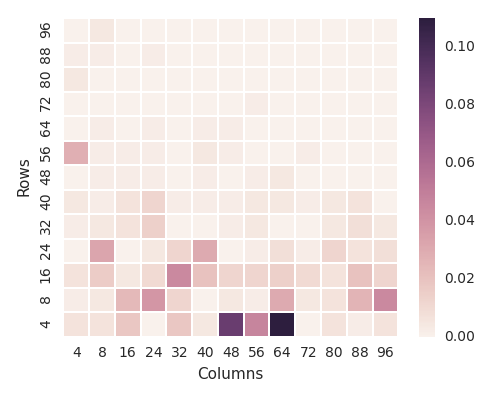
\includegraphics{gen/img/oracle_param_space.pdf}
\vspace{-1.5em} % Shrink vertical padding
\caption{}
\label{fig:oracle-wgsizes}
\end{subfigure}

\caption{%
  The distribution of: (\subref{fig:max-wgsizes}) maximum legal
  workgroup sizes, and (\subref{fig:oracle-wgsizes}) for all
  scenarios. The distribution of oracle workgroup sizes is uneven and
  spread across the space. \FIXME{These figures don't use the same
    scales.}%
}
\label{fig:heatmaps}
\end{figure}

Figure~\ref{fig:max-wgsizes} shows the distribution of maximum
workgroup sizes across all scenarios. Figure~\ref{fig:oracle-wgsizes}
shows the distribution of oracle workgroup sizes, demonstrating that
there is clearly no ``silver bullet'' workgroup size which works for
all scenarios. As Figure~\ref{fig:oracle-accuracy} shows,
\input{gen/num_wgsizes_50_accuracy} unique workgroup sizes are
required in order to achieve oracle performance just 50\% of the
time.

\begin{figure}
\centering
\includegraphics{gen/img/num_params_oracle.pdf}
\caption{%
  Accuracy compared to the oracle as a function of the number of
  workgroup sizes used. The best accuracy that is achievable using a
  single statically chosen value is
  \protect\input{gen/max_oracle_param_frequency}.%
}
\label{fig:oracle-accuracy}
\end{figure}

The mode of the oracle workgroup sizes is
\input{gen/max_oracle_param}, which is optimal for
\input{gen/max_oracle_param_frequency} of scenarios. Note that this is
a different value from the \emph{baseline} identified previously,
which identifies the single choice which provides the best average
case performance. This is because the value is not legal for all
scenarios; that is, $\input{gen/max_oracle_param_w} \not\in W_{safe}$.
Figure~\ref{fig:performance-legality} illustrates this point by
plotting the geometric mean performance across workgroup sizes for:
all scenarios, and only the scenarios for which the workgroup size is
legal.

\TODO{How many distinct oracle workgroup sizes are there?}

\TODO{What does the distribution of oracle workgroup sizes look like?}


\subsection{Human Expert}


The stencil workgroup size as chosen by a human expert is
$32 \times 4$.

\TODO{How often does this parameter fail?}

\TODO{When it is legal, how much of the available performance does
  this attain?}


\subsection{Heuristics}

\subsubsection{Per-device workgroup sizes}

\TODO{%
  What is the performance of picking one value per: architecture,
  dataset, and program?%
}

\subsubsection{Using maximum legal size}

A common approach taken by application developers is to set the
workgroup size for a kernel based on the maximum legal workgroup size,
for example to use the square root of the maximum to set the number of
columns and rows.

\TODO{What is the perforamnce of always picking the max legal value?}

\subsubsection{Scaling with maximum legal size}

% \TODO{Partial baseline. How much performance could we get if we lock
%   one of the parameters and twiddle the other?}

% While the reasoning for this approach is perfectly intuitive, these
% results indicate that there no useful correlation between the ratio
% of a particular workgroup size to the maximum legal workgroup and
% the observed performance.

\subsection{Summary}

By comparing the relative performance of an average of
\input{gen/avg_num_params} workgroup sizes for each workload, the
following conclusions can be drawn:

\begin{enumerate}
\item The performance of a workgroup size for a particular workload
  depends properties of the hardware, software, and dataset. The
  performance gap between different workgroup sizes for a single
  workload is up to $\input{gen/max_possible_speedup}\times$.
\item Not all workgroup sizes are legal, and we can only test if a
  value \emph{is} legal at runtime.
\item Differing workloads have wildly different optimal workgroup
  sizes, and the best performance can be achieved using static tuning
  is optimal for only \input{gen/max_oracle_param_frequency} of
  workloads.
\end{enumerate}

% I believe this presents a compelling case for the development of an
% autotuner which can select the optimal workgroup size at runtime.


\section{Classification Performance}


To evaluate the performance of a classifier, a subset of scenarios
$S_{training} \subset S$ are labelled with the workgroup size which
gave the best performance for each. The classifier is trained on this
labelled training data, and tested using a set of unseen scenarios
$S_{testing} = S - S_{training}$. The performance of each predicted
oracle workgroup size is compared against the true oracles for that
set. % Several selections of $S_{training}$ have been used:


\begin{figure}
\centering
\includegraphics{gen/img/ci_trend}
\caption{%
  % TODO: Use \input{gen/max_ci} and \input{gen/mean_ci}
  Ratio of confidence interval to mean as a function of sample
  count. The two dashed lines indicate the confidence interval at the
  minimum sample count (\fixme{4.5}\%), and mean sample count
  (\fixme{2.6}\%).%
}
\label{fig:ci-trends}
\end{figure}


\TODO{What is the distribution of runtimes?}

\TODO{Is the number of samples I have enough?}

\TODO{How does variance change with architecture, program, or
  dataset.}


\section{Optimising Workgroup Sizes}

% To begin to get a feel for the
%
% Figure~\ref{fig:performance-wgsizes}. Furthermore, the performance of
% workgroup sizes is shown in Figure~\ref{fig:performances} to be vary
% greatly across architectures, kernels, and datasets.

\TODO{What is the distribution of relative performance across
  architectures, programs, and datasets?}

\begin{table}
  \parbox{.45\linewidth}{
    \centering
    \scriptsize
    \rowcolors{2}{white}{gray!25}
    \input{gen/tab/top_params_coverage}
    \caption{The 25 workgroup sizes with the greatest legality.}
  }
  \hfill
  \parbox{.45\linewidth}{
    \centering
    \scriptsize
    \rowcolors{2}{white}{gray!25}
    \input{gen/tab/top_params_perf}
    \caption{The 25 workgroup sizes with the greatest performance.}
  }
\end{table}


\begin{figure}
\centering
\includegraphics{gen/img/params_summary.pdf}
\caption{%
  The red line shows the ``legality'' of workgroup sizes, i.e.\ the
  ratio of scenarios for which that workgroup size is legal.  The
  green lines show the geometric mean of the performance relative to
  the oracle for all scenarios for which the workgroup size is legal.%
}
\label{fig:performance-legality}
\end{figure}

\subsection{Refused Parameters}

Of the \input{gen/num_params} workgroup sizes tested,
\input{gen/ratio_refused_params}\% were refused in one or more test
cases, with an average \input{gen/ratio_refused_test_cases}\% of test
cases leading to refused parameters. For a workgroup size to be
refused, it must satisfy the architectural and program-specific
constraints which are exposed by OpenCL, but still lead to a
\texttt{CL\_OUT\_OF\_RESOURCES} error when the kernel is
enqueued. Table~\ref{tab:top-refused-params} lists the most frequently
refused parameters, and the percentage of test cases for which they
were refused. While uncommon, a refused parameters is an obvious
inconvenience to the user, as one would expect that any workgroup size
within the specified maximum should behave \emph{correctly} if not
performantly.

Figure~\ref{fig:refused-params-by-dev-vendor} suggests that the
problem is vendor --- or at least device --- specific. The
distribution of refused parameters is skewed towards the Intel CPU
devices, while no workgroup sizes were refused by the AMD
GPU. \TODO{Bug reports\ldots} For now, it is imperative that the
autotuning system be capable of adapting to these refused parameters
by suggesting alternatives when they occur.

\begin{table}
\parbox{.32\linewidth}{
    \centering
    \scriptsize
    \rowcolors{2}{white}{gray!25}
    \input{gen/tab/top_refused_params_1}
  }
  \hfill
  \parbox{.32\linewidth}{
    \centering
    \scriptsize
    \rowcolors{2}{white}{gray!25}
    \input{gen/tab/top_refused_params_2}
  }
  \hfill
  \parbox{.32\linewidth}{
    \centering
    \scriptsize
    \rowcolors{2}{white}{gray!25}
    \input{gen/tab/top_refused_params_3}
  }
  \caption{The thirty most refused parameters, ranked in descending
    order.}
  \label{tab:top-refused-params}
\end{table}

\begin{figure}
\centering
\begin{subfigure}[h]{.45\textwidth}
  \centering
  \includegraphics{gen/img/refused_params_by_device}
  \caption{}
  \label{fig:refused-params-by-device}
\end{subfigure}
\hfill
\begin{subfigure}[h]{.45\textwidth}
  \centering
  \includegraphics{gen/img/refused_params_by_vendor}
  \caption{}
  \label{fig:refused-params-by-vendor}
\end{subfigure}
\caption{%
  The ratio of test cases with refused workgroup sizes, grouped by:
  (\subref{fig:refused-params-by-device}) device;
  (\subref{fig:refused-params-by-vendor}) OpenCL vendor.%
}
\label{fig:refused-params-by-dev-vendor}
\end{figure}

% \begin{subfigure}[h]{.45\textwidth}
%   \centering
%   \includegraphics{gen/img/refused_param_space}
%   \caption{}
%   \label{fig:refused-params-space}
% \end{subfigure}


\cleardoublepage
\begin{figure}
\begin{subfigure}[h]{\textwidth}
\centering
\includegraphics{gen/img/performance_max_wgsize}
\vspace{-1.5em} % Shrink vertical padding
\caption{}
\label{fig:performance-max-wgsize}
\end{subfigure}
\\
\begin{subfigure}[h]{.48\textwidth}
\centering
\includegraphics{gen/img/performance_max_c}
\vspace{-1.5em} % Shrink vertical padding
\caption{}
\label{fig:performance-wg-c}
\end{subfigure}
~%
\begin{subfigure}[h]{.48\textwidth}
\centering
\includegraphics{gen/img/performance_max_r}
\vspace{-1.5em} % Shrink vertical padding
\caption{}
\label{fig:performance-wg-r}
\end{subfigure}

\caption{%
  Comparing workgroup performance relative to the oracle as function
  of: (\subref{fig:performance-max-wgsize})~maximum legal size,
  (\subref{fig:performance-wg-c})~number of columns, and
  (\subref{fig:performance-wg-r})~ number of rows.%
}
\label{fig:performance-wgsizes}
\end{figure}

\begin{figure}
\begin{subfigure}[h]{\textwidth}
\centering
\includegraphics{gen/img/performance_kernels.pdf}
\vspace{-1.5em} % Shrink vertical padding
\caption{Kernels}
\label{fig:performance-kernels}
\end{subfigure}
\\
\begin{subfigure}[h]{.48\textwidth}
\centering
\includegraphics{gen/img/performance_devices.pdf}
\vspace{-1.5em} % Shrink vertical padding
\caption{Devices}
\label{fig:performance-devices}
\end{subfigure}
~%
\begin{subfigure}[h]{.48\textwidth}
\centering
\includegraphics{gen/img/performance_datasets.pdf}
\vspace{-1.5em} % Shrink vertical padding
\caption{Datasets}
\label{fig:performance-datasets}
\end{subfigure}

\caption{%
  Performance relative to the oracle of workgroup sizes across all
  test cases, grouped by: (\subref{fig:performance-kernels})~kernels,
  (\subref{fig:performance-devices})~devices, and
  (\subref{fig:performance-datasets})~datasets.%
}
\label{fig:performances}
\end{figure}


\subsection{Performance Upper Bounds}

\begin{figure}
\includegraphics{gen/img/max_speedups}
\caption{%
  Speedup of oracle workgroup size over the worst workgroup size for
  each scenario, and the statically chosen workgroup size that
  provides the best overall performance.%
}
\label{fig:speedups}
\end{figure}

For a given scenario $s$, the ratio of the workgroups sizes from
$W_{legal}(s)$ which provide the longest and shortest mean runtimes is
used to calculate an upper bound for the possible performance
influence of workgroup size:

\begin{equation}
r_{max}(s) = r(s, \argmax_{w \in W_{legal}(s)} t(s,w), \Omega(s))
\end{equation}

When applied to each scenario $s \in S$ from the experimental results,
the average performance upper bound is found to be
$\input{gen/avg_possible_speedup}\times$ (range:
$\input{gen/min_possible_speedup}\times$ -
$\input{gen/max_possible_speedup}\times$).

\TODO{T-test to demonstrate confidence in differences between best and
  worst params.}


\subsection{Baseline Parameters}

From the experimental results, the baseline workgroup size $\bar{w}$
is found to be \input{gen/one_r}, with a geometric mean performance
$\bar{p}(\bar{w})$ of
\input{gen/one_r_perf}. Figure~\ref{fig:speedups} shows the speedup of
the oracle over this baseline parameter for all scenarios. If we
assume that a pragmatic developer with enough time would eventually
find this static optimal, then this provides a reasonable upper bound
on the attainable improvements of an autotuner for workgroup size over
that of a static choice.


\subsection{Oracle Workgroup Sizes}

\begin{figure}
\begin{subfigure}[t]{0.98\textwidth}
\centering
\includegraphics{gen/img/max_wgsizes.pdf}
\vspace{-1.5em} % Shrink vertical padding
\caption{}
\label{fig:max-wgsizes}
\end{subfigure}
\\
\begin{subfigure}[t]{0.98\textwidth}
\centering
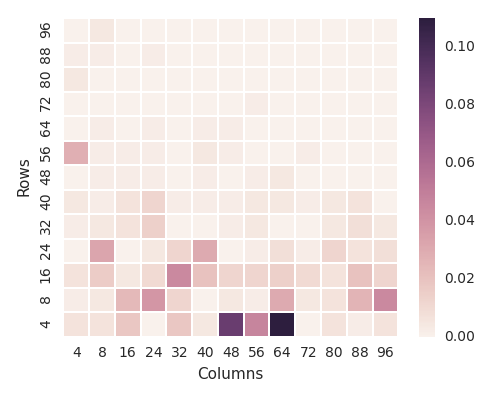
\includegraphics{gen/img/oracle_param_space.pdf}
\vspace{-1.5em} % Shrink vertical padding
\caption{}
\label{fig:oracle-wgsizes}
\end{subfigure}

\caption{%
  The distribution of: (\subref{fig:max-wgsizes}) maximum legal
  workgroup sizes, and (\subref{fig:oracle-wgsizes}) for all
  scenarios. The distribution of oracle workgroup sizes is uneven and
  spread across the space. \FIXME{These figures don't use the same
    scales.}%
}
\label{fig:heatmaps}
\end{figure}

Figure~\ref{fig:max-wgsizes} shows the distribution of maximum
workgroup sizes across all scenarios. Figure~\ref{fig:oracle-wgsizes}
shows the distribution of oracle workgroup sizes, demonstrating that
there is clearly no ``silver bullet'' workgroup size which works for
all scenarios. As Figure~\ref{fig:oracle-accuracy} shows,
\input{gen/num_wgsizes_50_accuracy} unique workgroup sizes are
required in order to achieve oracle performance just 50\% of the
time.

\begin{figure}
\centering
\includegraphics{gen/img/num_params_oracle.pdf}
\caption{%
  Accuracy compared to the oracle as a function of the number of
  workgroup sizes used. The best accuracy that is achievable using a
  single statically chosen value is
  \protect\input{gen/max_oracle_param_frequency}.%
}
\label{fig:oracle-accuracy}
\end{figure}

The mode of the oracle workgroup sizes is
\input{gen/max_oracle_param}, which is optimal for
\input{gen/max_oracle_param_frequency} of scenarios. Note that this is
a different value from the \emph{baseline} identified previously,
which identifies the single choice which provides the best average
case performance. This is because the value is not legal for all
scenarios; that is, $\input{gen/max_oracle_param_w} \not\in W_{safe}$.
Figure~\ref{fig:performance-legality} illustrates this point by
plotting the geometric mean performance across workgroup sizes for:
all scenarios, and only the scenarios for which the workgroup size is
legal.

\TODO{How many distinct oracle workgroup sizes are there?}

\TODO{What does the distribution of oracle workgroup sizes look like?}


\subsection{Human Expert}


The stencil workgroup size as chosen by a human expert is
$32 \times 4$.

\TODO{How often does this parameter fail?}

\TODO{When it is legal, how much of the available performance does
  this attain?}


\subsection{Heuristics}

\subsubsection{Per-device workgroup sizes}

\TODO{%
  What is the performance of picking one value per: architecture,
  dataset, and program?%
}

\subsubsection{Using maximum legal size}

A common approach taken by application developers is to set the
workgroup size for a kernel based on the maximum legal workgroup size,
for example to use the square root of the maximum to set the number of
columns and rows.

\TODO{What is the perforamnce of always picking the max legal value?}

\subsubsection{Scaling with maximum legal size}

% \TODO{Partial baseline. How much performance could we get if we lock
%   one of the parameters and twiddle the other?}

% While the reasoning for this approach is perfectly intuitive, these
% results indicate that there no useful correlation between the ratio
% of a particular workgroup size to the maximum legal workgroup and
% the observed performance.

\subsection{Summary}

By comparing the relative performance of an average of
\input{gen/avg_num_params} workgroup sizes for each workload, the
following conclusions can be drawn:

\begin{enumerate}
\item The performance of a workgroup size for a particular workload
  depends properties of the hardware, software, and dataset. The
  performance gap between different workgroup sizes for a single
  workload is up to $\input{gen/max_possible_speedup}\times$.
\item Not all workgroup sizes are legal, and we can only test if a
  value \emph{is} legal at runtime.
\item Differing workloads have wildly different optimal workgroup
  sizes, and the best performance can be achieved using static tuning
  is optimal for only \input{gen/max_oracle_param_frequency} of
  workloads.
\end{enumerate}

% I believe this presents a compelling case for the development of an
% autotuner which can select the optimal workgroup size at runtime.


\section{Classification Performance}


To evaluate the performance of a classifier, a subset of scenarios
$S_{training} \subset S$ are labelled with the workgroup size which
gave the best performance for each. The classifier is trained on this
labelled training data, and tested using a set of unseen scenarios
$S_{testing} = S - S_{training}$. The performance of each predicted
oracle workgroup size is compared against the true oracles for that
seTODO{What is the average speedup achieved using different
  classifiers?}

\TODO{What percentage of the maximum performance do the classifiers
  achieve?}

% \begin{figure}
% \centering
% \includegraphics{gen/img/classification-xval.pdf}
% \caption{%
%   Classification performance using cross-validation.%
% }
% \end{figure}

% \begin{figure}
% \centering
% \includegraphics{gen/img/classification-xval-random.pdf}
% \caption{%
%   Per-instance performances of classification using cross-validation
%   and the ``random'' error handler.%
% }
% \end{figure}


% \TODO{Rank eigenvectors of PCA on features.}

% \TODO{Evaluate the effectiveness of training with synthetic
%   benchmarks.}

\subsection{Selection of Features}

\TODO{How does the selection of features affect performance? Show a
  plot of performance vs number of features.}


\subsection{Effectiveness of Synthetic Benchmarks}

\TODO{How well does classification perform when trained solely on
  synthetic benchmarks, and tested soley on real benchmarks?}

\TODO{Repeat the above, but with incremtally fewere benchmarks.}


\subsection{Autotuning Overheads}

\TODO{What is the costs of auto-tuning?}

\TODO{How many iterations do we need to do before we ``break even''?}

% \section{Predicting Stencil Runtime}

% \begin{enumerate}
% \item How accurately does it predict the runtime of a stencil?
% \item What is the relationship between \emph{classification} accuracy,
%   and the accuracy of predicted runtimes? Does it really matter if the
%   predicted runtime is inaccurate?
% \end{enumerate}

% \begin{figure}
% \centering
% \includegraphics{gen/img/runtime-regression-xval.pdf}
% \caption{%
%   Performance of regressors at predicting program runtime.%
% }
% \end{figure}


% \section{Predicting Relative Performance}

\section{Comparison with hand tuned implementations}

\TODO{%
  Compare performance against some hand-crafted implementation of one
  of the real benchmarks.%
}


\section{Summary}

% \begin{table}
% \scriptsize
% \input{\DataDir/tab/xval.tex}
% \caption{Results of 10 fold cross-validation.}
% \end{table}

% \begin{table}
% \scriptsize
% \input{\DataDir/tab/synthetic_real.tex}
% \caption{Results of training using synthetic benchmarks and testing on
%   real.}
% \end{table}
